\section{Лабораторная работа 4 (Вариант 3)}
\subsection{Задание}

Выполнить классификацию двухмерных данных при помощи сети с самоорганизацией на основе конкуренции, обучающейся по алгоритму построения карты Кохонена.

\subsection{Описание сетей с самоорганизацией на основе конкуренции}
Сетями с самоорганизацией называются сети, не требующие для своего
обучения «учителя» и самостоятельно адаптирующие свои веса под обучающие
данные. Такие сети строятся из нейронов типа WTA и подобных
им. Как правило, это однослойные сети, в которых каждый нейрон получает
все компоненты входного вектора $X$ размерностью $N$. На рисунке \ref{img:schemeNet_lab3}
представлена структурная схема такой сети.

\begin{figure}[H]
\centering
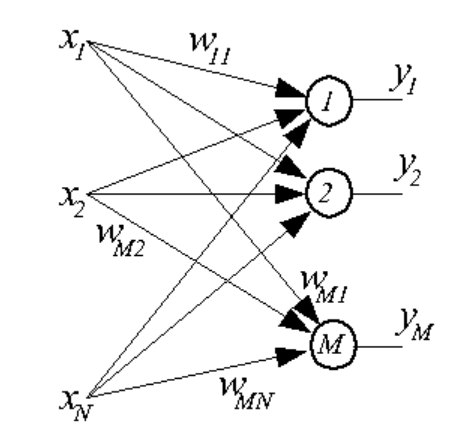
\includegraphics[scale=0.5]{schemeNet_lab3.png}
\caption{Схема сети с самоорганизацией на основе конкуренции}
\label{img:schemeNet_lab3}
\end{figure}

Веса входных связей $i$-ого нейрона образуют вектор
\begin{equation}
    W_{i} = \left[ \begin{array} { l l l l }{w_{i 1}} & {w_{i 2}}&{\dots}&{w_{ i N }}\end{array}\right]^{T} .
\end{equation}

Кроме связей, явно представленных в схеме, на этапе обучения имеют место
связи между нейронами, позволяющие судить о степени «соседства»
нейронов друг с другом, при этом смысл понятия «соседство» может
быть разным.
Укрупненно процесс обучения сети выглядит следующим образом. На
вход сети подается обучающий вектор $X^k$, для каждого нейрона определяется
$d(X^k, W_i)$ — расстояние (в смысле выбранной метрики) между
векторами Xk и Wi. Определяется нейрон–победитель, для которого это
расстояние оказывается наименьшим. Вокруг нейрона–победителя образуется окрестность $S^k_w$ из нейронов–соседей с известным «расстоянием» до победителя. Веса нейрона–победителя и веса его соседей из $S^k_w$ уточняются, например, по правилу Кохонена:

\begin{equation}
	W_{i}^{k+1} = W_{i}^{k}+\eta_{i}^{k}\left(X^{k}-W_{i}^{k}\right) ,
\end{equation}

где $\eta^k_i$ --- коэффициент обучения, значение которого уменьшается с увеличением расстояния от $i$-ого нейрона до победителя. Веса нейронов вне $S^k_w$ не изменяются. Размер окрестности $S^k_w$ и величина $\eta^k_i$ с течением времени обучения уменьшаются.

В качестве меры измерения расстояния между векторами чаще всего
используются:
\begin{itemize}
\item евклидова мера $d \left( X , W _ { i } \right) = \left\| X - W _ { i } \right\| = \sqrt { \sum _ { j = 1 } ^ { N } \left( x _ { j } - w _ { i j } \right) ^ { 2 } }$
\item скалярное произведение
$d \left( X , W _ { i } \right) = 1 - X \cdot W _ { i } = 1 - \| X \| _ { 2 } \cdot \left\| W _ { i } \right\| _ { 2 } \cdot \cos \left( \angle X W _ { i } \right)$

\item манхэттеновское расстояние $d \left( X , W _ { i } \right) = \sum _ { j = 1 } ^ { N } \left| x _ { j } - w _ { i j } \right|$;

\item m-норма $d \left( X , W _ { i } \right) = \max _ { j } \left| x _ { j } - w _ { i j } \right|$.
\end{itemize}

\subsection{Решение проблемы мертвых нейронов}
\label{seq:deadNeurons}
При «слепом» (как правило, случайном) выборе начальных значений весов
часть нейронов может оказаться в области пространства, в которой
отсутствуют обучающие данные или где их количество ничтожно мало.
Такие нейроны имеют очень мало шансов на победу в конкурентной
борьбе и адаптацию своих весов, вследствие чего они остаются мертвыми.
В итоге уменьшается количество активных нейронов, участвующих
в анализе входных данных, и, следовательно, увеличивается погрешность
их интерпретации, называемая погрешностью квантования. Встает проблема
активации всех нейронов сети на этапе обучения.
Такую активацию можно осуществить, базируясь на учете количества
побед, одержанных каждым нейроном в ходе обучения. Существуют
разные механизмы такого учета.
В одном из таких подходов каждому нейрону сети приписывается
потенциал $\pi_i$
, значение которого модифицируется после предъявления
каждого обучающего вектора $X^k$ по следующей формуле (в ней $w$ —
индекс нейрона-победителя):

\begin{equation}\label{eq:system}
		\begin{aligned}
		&	\pi _ { i } ^ { k + 1 } = \pi _ { i } ^ { k } + 1 / M, где i \neq w\\
		&   \pi _ { i } ^ { k + 1 } = \pi _ { i } ^ { k } - \pi _ { min }, где i = w.
		\end{aligned}  		
\end{equation}

где $\pi_{min}$ — минимальный потенциал, разрешающий участие в конкурентной борьбе. Максимальное значение потенциала устанавливается равным 1. На практике хорошие результаты получены для $\pi_{min} = 0.75$ .

Целью обучения сети с самоорганизацией на основе конкуренции является минимизация погрешности квантования:

\begin{equation}
 E _ { q } = \frac { 1 } { p } \sum _ { k = 1 } ^ { p } d \left( X ^ { k } , W _ { w ( k ) } \right)
\end{equation}

где $p$ — количество обучающих векторов $X^k$, $W_{w(k)}$ — вектор весов нейрона–победителя при предъявлении вектора $X^k$.
Примеры результатов обучения, близких к оптимальным, представлены
ниже на рисунках. Используются сети с 15 и 22 нейронами и двухкомпонентным входным вектором $X = \left[ x _ { 1 } , x _ { 2 } \right] ^ { T }$. На левых картинках (рисунок \ref{img:somNetr}) представлено распределение данных в обучающих выборках, на правых --- распределение весов нейронов обученной сети.

\begin{figure}[H]
\centering
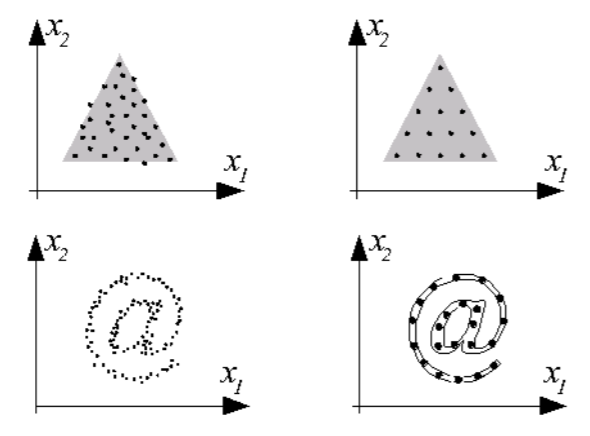
\includegraphics[scale=0.5]{somNet.png}
\caption{Схема сети с самоорганизацией на основе конкуренции}
\label{img:somNetr}
\end{figure}

В нейронных сетях, предложенных Т. Кохоненом (1982 г.), соседство нейронов
носит чисто топологический характер. В простом случае нейроны
слоя Кохонена образуют одномерную цепочку, при этом каждый нейрон
имеет, в общем случае, двух ближайших соседей (слева и справа).
В более сложном случае нейроны Кохонена образуют двумерную сетку
с четырьмя соседями у каждого нейрона (слева, справа, сверху, снизу).
В еще более сложном случае сетка гексагональна — у каждого нейрона
шесть соседей на плоскости (по циферблату часов — 2, 4, 6, 8, 10, 12
часов).
Коррекция весов нейронов в ходе обучения выполняется по формуле

\begin{equation}
W _ { i } ^ { k + 1 } = W _ { i } ^ { k } + \eta ^ { k } G ^ { k } \left( i , X ^ { k } \right) \left( X ^ { k } - W _ { i } ^ { k } \right),
\end{equation}


где функция соседства $G ^ { k } \left( i , X ^ { k } \right)$ определяется, как правило, формулой Гаусса в вид

\begin{equation}
G ^ { k } \left( i , X ^ { k } \right) = \exp \left( - \frac { d ^ { 2 } \left( i , X ^ { k } \right) } { 2 \left( \sigma ^ { k } \right) ^ { 2 } } \right),
\end{equation}

где $d \left( i , X ^ { k } \right)$ ---  расстояние от $i$-ого нейрона до нейрона–победителя с индексом $w_k$ в $k$-ом цикле обучения. При этом $d \left( w ^ { k } , X ^ { k } \right) = 0 , d \left( i , X ^ { k } \right) = 1$ для всех ближайших соседей $w_k$, $d(i, X^k) = 2$ для всех «внешних» ближайших соседей ближайших соседей нейрона победителя с индексом $w^k$ и так далее.

Как обычно, коэффициент обучения $\eta^k$ и параметр ширины функции
Гаусса $\sigma^k$ уменьшаются в ходе обучения (с ростом $k$). В результате обучения слоя Кохонена по такому алгоритму топологически
соседние нейроны становятся типичными представителями кластеров обучающих данных, соседствующих в многомерном пространстве.
В этом достоинство сетей Кохонена, называемых также картами Кохонена, — наглядность в представлении (путем одномерной или двумерной
визуализации) многомерных данных.

Очевидным практическим приложением сетей с самоорганизацией является
сжатие (с потерями) данных, в частности, покадровое сжатие изображений.
Но мы воспользуемся ей для других целей.
Важным свойством сетей с самоорганизацией на основе конкуренции
является способность к кластеризации данных и их распознаванию. Это
обеспечивает их широкое применение для решения задач диагностики,
например, неисправностей оборудовани


\subsection{Реализация}

В качестве топологии сети выбрана линейная топология, т.е соседство нейронов определяется близостью их порядкового номера. При случайном разбросе начальных весов на примере пяти нейронов, соседство выглядит следующим образом (нейроны-соседи первого порядка соединены линиями).

\begin{figure}[H]
\centering
\includegraphics[scale=0.5]{topologyNet.png}
\caption{Демострация топологии соседства при случаном разбросе пяти нейронов в двухмерном пространстве параметров}
\label{img:somNetr}
\end{figure}

При проверке очередного вектора $X^k$ из обучающей выборки, определяется евклидово расстояние между данным вектором и каджым из  нейронов:
\begin{equation}
    d \left( X , W _ { i } \right) = \left\| X - W _ { i } \right\| = \sqrt { \sum _ { j = 1 } ^ { N } \left( x _ { j } - w _ { i j } \right) ^ { 2 } }
\end{equation}

Среди них находится наименьшее расстояние $d_{min} = \min d \left( X^k , W _ { i } \right), i = 1, ..., M$. 

Для корректировки весов нейрона-победителя и нейронов-соседей используется формула:
\begin{equation}
W _ { i } ^ { k + 1 } = W _ { i } ^ { k } + \eta ^ { k } G ^ { k } \left( i , X ^ { k } \right) \left( X ^ { k } - W _ { i } ^ { k } \right),
\end{equation}

где функция соседства $G ^ { k } \left( i , X ^ { k } \right)$ определяется, как правило, формулой Гаусса в вид

\begin{equation}
G ^ { k } \left( i , X ^ { k } \right) = \exp \left( - \frac { d ^ { 2 } \left( i , X ^ { k } \right) } { 2 \left( \sigma ^ { k } \right) ^ { 2 } } \right),
\end{equation}

где 
\begin{equation}
	d(i, X^k) = \left| i - w \right|,
\end{equation}

где $i$ --- номер текущего нейрона, $w$ --- индекс нейрона-победителя. Таким образом, по мере отдаления от нейрона-победителя коррекция веса нейрона спадает.

По мере увеличения времени, значения коэффициентов $\eta ^ { k }$ и $\sigma ^ { k }$ должны уменьшаться. В данной работе, по причине простоты подбора параметров, принято линейное убывание этих коэффициентов при увеличении времени:

\begin{equation}\label{eq:linearDecay}
		\begin{aligned}
		&	\sigma (t) = \dfrac{\sigma_{min} - \sigma_{max}}{t_{max} - 1}(t - 1) + \sigma_{max},\\
		&   \eta (t) = \dfrac{\eta_{min} - \eta_{max}}{t_{max} - 1}(t - 1) + \eta_{max}.
		\end{aligned}  		
\end{equation}

При этом значение $\eta = 0 ... 1$, то есть изменяя параметр $\eta_{min}$ мы меняем величину наклона линии (график $\eta (t)$) и, следовательно, скорость уменьшения параметра. Величина $\sigma$ может принимать произвольные значения.

Проблема мертвых нейронов на начальном этапе обучения решается путем введения потенциалов по процедуре, описанной в разделе \ref{seq:deadNeurons}. 
Минимальный потенциал принимается равным $\pi_{min} = 0.75$ и присваивается изначально всем нейронам.

\subsection{Обучение}
Выборка, на которой происходит обучение, и первоначальное расположение 16-ти нейронов показаны на рисунке  \ref{img:startpos}.

\begin{figure}[H]
\centering
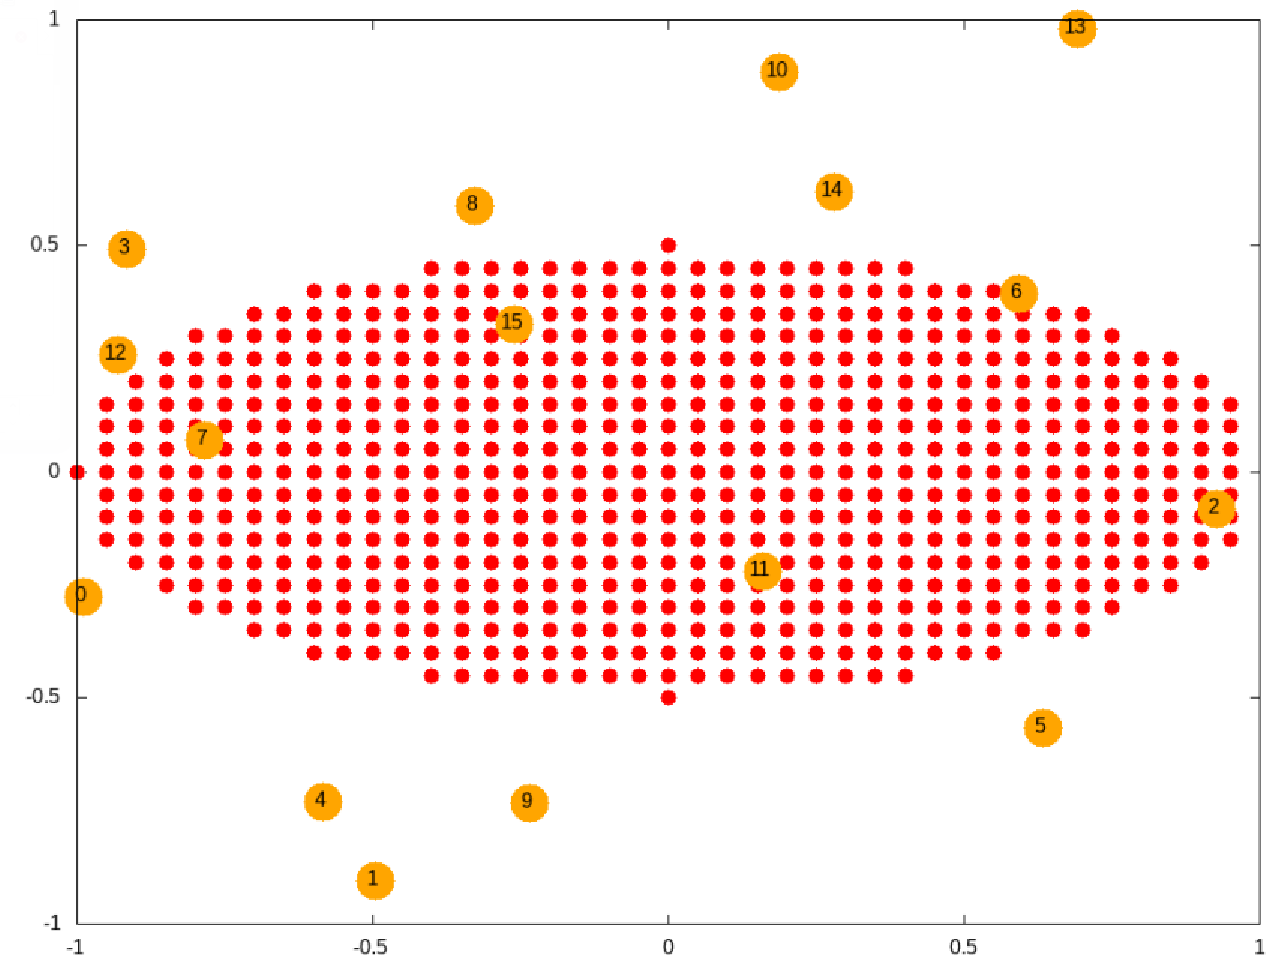
\includegraphics[scale=0.3]{startpos.png}
\caption{Обучающая выборка и расположение весов при инициализации}
\label{img:startpos}
\end{figure}

Веса разыграны по равномерному распределению вдоль каждой координатной оси в диапазоне от 0 до 1: $w_{ik} = Uniform(-1;1)$, где $Uniform(a, b)$ --- функция равномерного распределения на отрезке $[a;b]$.

Для того, чтобы дать каждому нейрону возможность проявить себя и ликвидировать мертвые нейроны, произведено $M = 16$ итерации предварительного обучения. 

Значения параметров:
\begin{equation}
	\begin{aligned}
	 &	\sigma_{min} = 0.5,  \\ 
	 &	\sigma_{max} = 2.1, \\	
	 &	\eta_{min} = 0.5,  \\ 
	 &	\eta_{max} = 1, \\
	\end{aligned}
\end{equation} 

В результате, нейроны расположились следующим образом:

\begin{figure}[H]
\centering
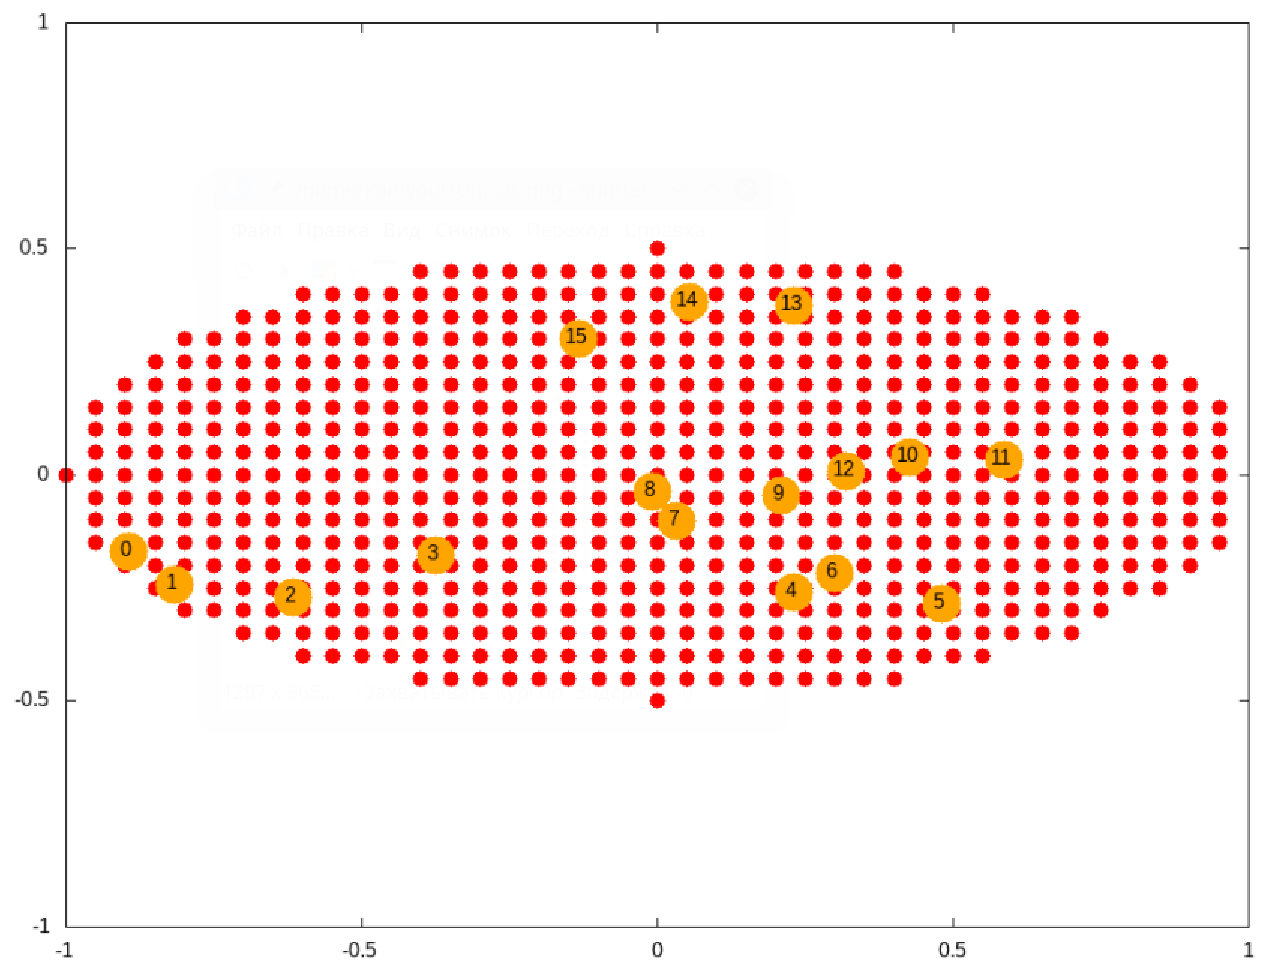
\includegraphics[scale=0.3]{afterPreTrain.png}
\caption{Расположение нейронов после предварительного обучения ("оживления")}
\label{img:afterPreTrain}
\end{figure}

Для полноценного обучения, при котором больше не происходит изменения потенциалов нейронов, произведен обход входных данных в 10 эпох. Завершение работы алгоритма происходит при окончании всех эпох обучения, без учета минимизации величины ошибки квантования.
Параметры при этом заданы следующие:

\begin{equation}
	\begin{aligned}
	 &	\sigma_{min} = 0.01,  \\ 
	 &	\sigma_{max} = 1., \\	
	 &	\eta_{min} = 0.001,  \\ 
	 &	\eta_{max} = 0.5, \\
	\end{aligned}
\end{equation}

Результирующее распределение нейронов:

\begin{figure}[H]
\centering
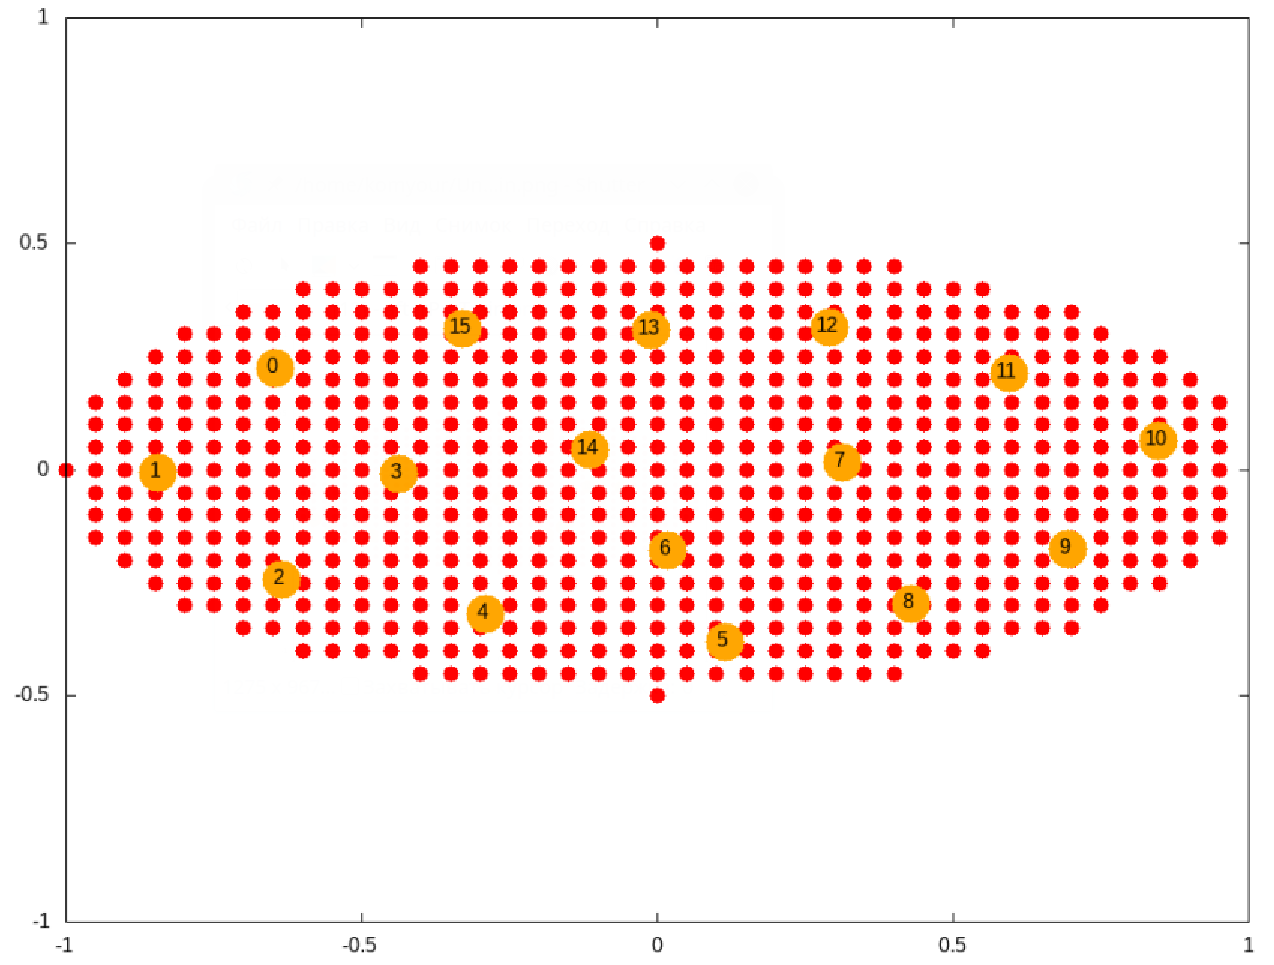
\includegraphics[scale=0.3]{finalpos.png}
\caption{Расположение нейронов после предварительного обучения ("оживления")}
\label{img:finalpos}
\end{figure}

\subsection{Вывод}

По рисунку \ref{img:finalpos} видно, что в результате обучения нейроны расположились равномерно по обучающей выборке, при этом соседние (по топологии сети) нейроны находятся рядом и на множестве обучающих данных, что говорит о правльности реализации алгоритма Кохонена.

При предварительном обучении исходные параметры $\sigma_{min}$, $\sigma_{max}$, $\eta_{min}$, $\eta_{max}$ следует подбирать таким образом, чтобы за небольшое количество итераций "оживить все нейроны". Достигается это за счет большого значения $\sigma_{max} = 1.9 .. 2.6 $ при  $\sigma_{min} = 0.5 .. 0.8$. Начальное значение $\eta_{max} = 1$, для более резкой подстройки весов на старте обучения, $\eta_{min} = 0.55 .. 0.3$.

В основном цикле обучения выполняется более тонкая настройка весов, поэтому значения параметров $\sigma_{max} = 1.1 .. 0.6 $,  $\sigma_{min} = 0.01 .. 0.001$, $\eta_{max} = 0.6 .. 0.3$, $\eta_{min} = 0.001 .. 0.0001$ значительно меньше, по сравнению с предварительным этапом.

\subsection{Код программы}
Файл main.cpp.
\begin{verbatim}
     1  #include "NetSOM.h"
     2  #include <algorithm>
     3  #include <cmath>
     4  #include <random>
     5
     6  void GenerateElipsoid (
     7          std::vector<std::vector<double>> *points,
     8          double a, double b,
     9          double xOffset, double yOffset,
    10          double rotation, double step) 
    11  {
    12      a = (a < 0) ? -a : a;
    13      b = (b < 0) ? -b : b;
    14      for (double x = -a; x <= a; x += step) {
    15          for (double y = -b; y <= b; y += step) {
    16               if (((x * x) / (a * a) + (y * y) / (b * b)) <= 1)
 {
    17                  std::vector<double> v(2);
    18                  v[0] = ( x * cos(rotation) + y * sin(rotation)
) + xOffset;
    19                  v[1] = (-x * sin(rotation) + y * cos(rotation)
) + yOffset;
    20                  points->emplace_back(std::move(v));
    21               }
    22          }
    23      }
    24  }
    25
    26  void SaveTrainSetToFile(std::ostream &output, const std::vecto
r<std::vector<double>> &points) {
    27      for (size_t iPoint = 0; iPoint < points.size(); ++iPoint) 
{
    28          for (size_t iCoord = 0; iCoord < points[iPoint].size()
; ++iCoord)
    29              output << points[iPoint][iCoord] << "\t";
    30          output << std::endl;
    31      }
    32  }
    33
    34  int main() {
    35      std::vector<std::vector<double>> trainSet;
    36      GenerateElipsoid (&trainSet, 1., 0.5, 0., 0., 0., 0.05);
    37      NetSOM  net;
    38      NetSOM::NetConfig netConf;
    39
    40      netConf.neurons  = 16;
    41      netConf.inVecDim = 2;
    42      netConf.trainEpochs = 10.;
    43      netConf.preTrainIterations = netConf.neurons;
    44      netConf.minPotential = 0.25;
    45      netConf.deltaMinFuncEps = 1e-3;
    46
    47      netConf.sigmaInitPreTrain = 2.1;
    48      netConf.sigmaInitPreTrainMin = 0.5;
    49      netConf.etaInitPreTrain = 1.;
    50      netConf.etaInitPreTrainMin = 0.5;
    51
    52      netConf.sigmaInit = 1.;
    53      netConf.sigmaInitMin = 1e-1;
    54      netConf.etaInit = 0.5;
    55      netConf.etaInitMin = 1e-3;
    56      netConf.weightLowBound   = -1.;
    57      netConf.weightUpperBound =  1.;
    58
    59      netConf.weightFileName = std::string("weight.data");
    60
    61      net.Init(netConf);
    62
    63      std::ofstream trainSetFile("train.data", std::ios::trunc);
    64      std::ofstream weightFile(netConf.weightFileName, std::ios:
:trunc);
    65      std::ofstream gnuplotFile("plot.txt", std::ios::trunc);
    66      SaveTrainSetToFile(trainSetFile, trainSet);
    67      net.Train(trainSet, weightFile);
    68      net.CreateGnuplotAnimation(gnuplotFile);
    69      std::cerr << "End of training " << std::endl;
    70  }
\end{verbatim}

Файл NetSOM.h

\begin{verbatim}
     1  #include <vector>
     2  #include <iostream>
     3  #include <fstream>
     4  using size_t = std::size_t;
     5
     6  class NetSOM {
     7  public:
     8      struct NetConfig {
     9          size_t neurons;
    10          size_t inVecDim;
    11          int    trainEpochs;
    12          int    preTrainIterations;
    13          double minPotential;
    14          double deltaMinFuncEps;
    15          
    16          double sigmaInitPreTrain;
    17          double etaInitPreTrain;
    18          double sigmaInitPreTrainMin;
    19          double etaInitPreTrainMin;
    20          
    21          double sigmaInit;
    22          double etaInit;
    23          double sigmaInitMin;
    24          double etaInitMin;
    25
    26          double weightLowBound;
    27          double weightUpperBound;
    28
    29          std::string weightFileName;
    30      };
    31      void Init(const NetConfig &conf);
    32      size_t DetectWinner(const std::vector<double> &inVec);
    33
    34      void Train(std::vector<std::vector<double>> &trainSet,
    35                 std::ostream &outputLabels);
    36
    37      void PrintWeightsToFile(std::ostream &output, int precisio
n);
    38      void CreateGnuplotAnimation(std::ofstream &stream);
    39  private:
    40      NetConfig netConfig;
    41      std::vector<double>   weights;
    42      std::vector<double>   potential;
    43      double sigma;
    44      double eta;
    45      void RandomWeights();
    46      void AdjustWeights(size_t winnerInd, const std::vector<dou
ble> &inVec);
    47      void AdjustPotential(size_t winnerInd);
    48  };
\end{verbatim}

Файл NetSOM.cpp
\begin{verbatim}
     1  #include "NetSOM.h"
     2  #include <iomanip>
     3  #include <random>
     4  #include <algorithm>
     5  #include <limits>
     6  #include <fstream>
     7
     8  void NetSOM::Init(const NetConfig &conf) {
     9      netConfig = conf;
    10      weights.resize(netConfig.neurons * netConfig.inVecDim);
    11      potential.resize(netConfig.neurons, netConfig.minPotential
);
    12      RandomWeights();
    13  }
    14  // -----------------------------------------------------------
-------------------------------------
    15  void NetSOM::RandomWeights() {
    16      std::random_device randomizer;
    17      std::mt19937 randGen(randomizer());
    18      std::uniform_real_distribution<> dist(netConfig.weightLowB
ound, 
    19                                            netConfig.weightUppe
rBound);
    20      double weightNorm;
    21      double weight = 0.0;
    22      for (size_t iNeuron = 0; iNeuron < netConfig.neurons; ++iN
euron) {
    23          for (size_t iWeight = 0; iWeight < netConfig.inVecDim;
 ++iWeight) {
    24              weight = dist(randGen);
    25              std::cerr << weight << std::endl;
    26              weights[iWeight + iNeuron * netConfig.inVecDim] = 
weight;
    27          }
    28      }
    29  }
    30  // -----------------------------------------------------------
-------------------------------------
    31  // returns winner index
    32  size_t NetSOM::DetectWinner(const std::vector<double> &inVec) 
{
    33      std::vector<double> distancesToInput(netConfig.neurons, 0.
0);
    34      
    35      for (size_t iNeuron = 0; iNeuron < netConfig.neurons; ++iN
euron) {
    36          for (size_t iWeight = 0; iWeight < netConfig.inVecDim;
 ++iWeight) {
    37              distancesToInput[iNeuron] += pow(inVec[iWeight] - 
weights[iWeight + iNeuron * netConfig.inVecDim], 2);        
    38          }
    39          if (potential[iNeuron] < netConfig.minPotential) {
    40              distancesToInput[iNeuron] = std::numeric_limits<do
uble>::max();
    41          } else {
    42              distancesToInput[iNeuron] = potential[iNeuron] * s
qrt(distancesToInput[iNeuron]);
    43          }
    44      }
    45      size_t winnerInd = std::distance(distancesToInput.begin(),
 std::min_element(distancesToInput.begin(), distancesToInput.end()));
    46      return winnerInd;
    47  }
    48  // -----------------------------------------------------------
-------------------------------------
    49  void NetSOM::AdjustWeights(size_t winnerInd, const std::vector
<double> &inVec) {
    50      for (size_t iNeuron = 0; iNeuron < netConfig.neurons; ++iN
euron) {
    51          for (size_t iWeight = 0; iWeight < netConfig.inVecDim;
 ++iWeight) {
    52              double d = abs(iNeuron - winnerInd);
    53              double neigbourCoeff = exp(-pow(d / sigma, 2) / 2)
;
    54              weights[iWeight + iNeuron * netConfig.inVecDim] +=
 eta * neigbourCoeff 
    55                                                                
  * (inVec[iWeight] - weights[iWeight + iNeuron * netConfig.inVecDim])
;
    56          }
    57      }
    58  }
    59  // -----------------------------------------------------------
-------------------------------------
    60  void NetSOM::AdjustPotential(size_t winnerInd) {
    61      for (size_t iPotential = 0; iPotential < potential.size();
 iPotential++) {
    62          (iPotential == winnerInd) ? potential[iPotential] -= n
etConfig.minPotential
    63                                  : potential[iPotential] += 1. 
/ netConfig.neurons;
    64          std::cout << potential[iPotential] << std::endl;
    65      }
    66  }
    67  // -----------------------------------------------------------
-------------------------------------
    68  void NetSOM::Train(std::vector<std::vector<double>> &trainSet,
    69                       std::ostream &outputLabels) 
    70  {
    71      size_t winnerInd;
    72      double maxT;
    73      // pretraining stage: solves problem of dead neurons
    74      std::random_shuffle(trainSet.begin(), trainSet.end());
    75      PrintWeightsToFile(outputLabels, 16);
    76      for (size_t iVec = 0; iVec < netConfig.preTrainIterations;
 ++iVec) {
    77          double time = (iVec + 1);        
    78          sigma = (netConfig.sigmaInitPreTrainMin - netConfig.si
gmaInitPreTrain) 
    79                / (netConfig.preTrainIterations - 1) * (time - 1
) + netConfig.sigmaInitPreTrain;
    80          eta   = (netConfig.etaInitPreTrainMin   - netConfig.et
aInitPreTrain)   
    81                / (netConfig.preTrainIterations - 1) * (time - 1
) + netConfig.etaInitPreTrain;
    82          winnerInd = DetectWinner(trainSet[iVec]);
    83          AdjustPotential(winnerInd);
    84          AdjustWeights(winnerInd, trainSet[iVec]);
    85          PrintWeightsToFile(outputLabels, 16);
    86      }
    87      // adjust potential of each neuron equals to 1.
    88      for (int iPot = 0; iPot < potential.size(); iPot++) {
    89          potential[iPot] = 1.;
    90      }
    91      maxT = netConfig.trainEpochs * trainSet.size();
    92      double time = 0.;
    93      for (size_t iEpoch = 0; iEpoch < netConfig.trainEpochs; ++
iEpoch) {
    94          std::random_shuffle(trainSet.begin(), trainSet.end());
    95          for (size_t iVec = 0; iVec < trainSet.size(); ++iVec) 
{
    96              time++;
    97              sigma = (netConfig.sigmaInitMin - netConfig.sigmaI
nit) / (maxT - 1) * (time - 1) + netConfig.sigmaInit;
    98              eta   = (netConfig.etaInitMin - netConfig.etaInit)
     / (maxT - 1) * (time - 1) + netConfig.etaInit;
    99              winnerInd = DetectWinner(trainSet[iVec]);
   100              AdjustWeights(winnerInd, trainSet[iVec]);
   101              PrintWeightsToFile(outputLabels, 16);
   102          }
   103      }
   104  }
   105  // -----------------------------------------------------------
-------------------------------------
   106  void NetSOM::PrintWeightsToFile(std::ostream &output, int prec
ision) {
   107      for (size_t iWeight = 0; iWeight < weights.size(); ++iWeig
ht) {
   108          output << std::setprecision(precision) << weights[iWei
ght] << "\t";
   109          if (iWeight % 2) {
   110              output << iWeight / netConfig.inVecDim << "\t";
   111          }
   112      }
   113      output << std::endl << std::endl << std::endl;
   114  }
   115  // -----------------------------------------------------------
-------------------------------------
   116  void NetSOM::CreateGnuplotAnimation(std::ofstream &stream) {
   117      stream << " set terminal gif size 1024, 768 animate delay 
0.001 loop -1 "<< std::endl
   118                << " set output 'train.gif' "<< std::endl
   119                << " set xrange [-1:1] "<< std::endl
   120                << " set yrange [-1:1] "<< std::endl
   121                << " unset key "<< std::endl              
   122                << " stats \'" << netConfig.weightFileName << "\
' nooutput  "<< std::endl
   123                << " do for [i=1:int(STATS_blocks)-1] { "<< std:
:endl
   124                << "     plot \"points.data\" index 0 using 1:2 
pt 7 ps 2 lc rgb \'red\',\\"<< std::endl;
   125      for (size_t iNeuron = 0; iNeuron < netConfig.neurons - 1; 
iNeuron++) {
   126          stream << "      \"" << netConfig.weightFileName <<"\"
 index(i-1) using " 
   127                 <<  (iNeuron+1)*3 - 2 << ":" << (iNeuron+1)*3 -
 1
   128                 << "  pt 7 ps 5 lc rgb \'orange\',\\"<< std::en
dl;
   129          stream << "      \"" << netConfig.weightFileName <<"\"
 index(i-1) using " 
   130                 <<  (iNeuron+1)*3 - 2 << ":" << (iNeuron+1)*3 -
 1 << ":" << (iNeuron+1)*3
   131                 << "  with labels,\\"<< std::endl;
   132      }
   133      stream << "      \"" << netConfig.weightFileName <<"\" ind
ex(i-1) using " 
   134             <<  (netConfig.neurons)*3 - 2 << ":" << (netConfig.
neurons)*3 - 1
   135             << "  pt 7 ps 5 lc rgb \'orange\',\\"<< std::endl;
   136      stream << "      \"" << netConfig.weightFileName <<"\" ind
ex(i-1) using " 
   137             <<  (netConfig.neurons)*3 - 2 << ":" << (netConfig.
neurons)*3 - 1 << ":" << (netConfig.neurons)*3
   138             << "  with labels\\"<< std::endl;
   139      stream << "}" << std::endl;
   140
   141      std::ofstream file;
   142      file.open("finalpos.txt", std::ios::trunc);
   143      file << " set terminal gif size 1024, 768 animate delay 0.
001 loop -1 "<< std::endl
   144                << " set output 'final.gif' "<< std::endl
   145                << " set xrange [-1:1] "<< std::endl
   146                << " set yrange [-1:1] "<< std::endl
   147                << " unset key "<< std::endl              
   148                << " stats 'weight.data' nooutput  "<< std::endl
   149                << " do for [i=int(STATS_blocks)-1:int(STATS_blo
cks)-1] { "<< std::endl
   150                << "     plot \"points.data\" index 0 using 1:2 
pt 7 ps 2 lc rgb \'red\',\\"<< std::endl;
   151      for (size_t iNeuron = 0; iNeuron < netConfig.neurons - 1; 
iNeuron++) {
   152          file << "      \"" << netConfig.weightFileName <<"\" i
ndex(i-1) using " 
   153                 <<  (iNeuron+1)*3 - 2 << ":" << (iNeuron+1)*3 -
 1
   154                 << "  pt 7 ps 5 lc rgb \'orange\',\\"<< std::en
dl;
   155          file << "      \"" << netConfig.weightFileName <<"\" i
ndex(i-1) using " 
   156                 <<  (iNeuron+1)*3 - 2 << ":" << (iNeuron+1)*3 -
 1 << ":" << (iNeuron+1)*3
   157                 << "  with labels,\\"<< std::endl;
   158      }
   159      file << "      \"" << netConfig.weightFileName <<"\" index
(i-1) using " 
   160             <<  (netConfig.neurons)*3 - 2 << ":" << (netConfig.
neurons)*3 - 1
   161             << "  pt 7 ps 5 lc rgb \'orange\',\\"<< std::endl;
   162      file << "      \"" << netConfig.weightFileName <<"\" index
(i-1) using " 
   163             <<  (netConfig.neurons)*3 - 2 << ":" << (netConfig.
neurons)*3 - 1 << ":" << (netConfig.neurons)*3
   164             << "  with labels\\"<< std::endl;
   165      file << "}" << std::endl;
   166
   167      std::ofstream fileStart;
   168      fileStart.open("startpos.txt", std::ios::trunc);
   169      fileStart << " set terminal gif size 1024, 768 animate del
ay 0.001 loop -1 "<< std::endl
   170                << " set output 'startpos.gif' "<< std::endl
   171                << " set xrange [-1:1] "<< std::endl
   172                << " set yrange [-1:1] "<< std::endl
   173                << " unset key "<< std::endl              
   174                << " stats 'weight.data' nooutput  "<< std::endl
   175                << " do for [i=1:1] { "<< std::endl
   176                << "     plot \"points.data\" index 0 using 1:2 
pt 7 ps 2 lc rgb \'red\',\\"<< std::endl;
   177      for (size_t iNeuron = 0; iNeuron < netConfig.neurons - 1; 
iNeuron++) {
   178          fileStart << "      \"" << netConfig.weightFileName <<
"\" index(i-1) using " 
   179                 <<  (iNeuron+1)*3 - 2 << ":" << (iNeuron+1)*3 -
 1
   180                 << "  pt 7 ps 5 lc rgb \'orange\',\\"<< std::en
dl;
   181          fileStart << "      \"" << netConfig.weightFileName <<
"\" index(i-1) using " 
   182                 <<  (iNeuron+1)*3 - 2 << ":" << (iNeuron+1)*3 -
 1 << ":" << (iNeuron+1)*3
   183                 << "  with labels,\\"<< std::endl;
   184      }
   185      fileStart << "      \"" << netConfig.weightFileName <<"\" 
index(i-1) using " 
   186             <<  (netConfig.neurons)*3 - 2 << ":" << (netConfig.
neurons)*3 - 1
   187             << "  pt 7 ps 5 lc rgb \'orange\',\\"<< std::endl;
   188      fileStart << "      \"" << netConfig.weightFileName <<"\" 
index(i-1) using " 
   189             <<  (netConfig.neurons)*3 - 2 << ":" << (netConfig.
neurons)*3 - 1 << ":" << (netConfig.neurons)*3
   190             << "  with labels\\"<< std::endl;
   191      fileStart << "}" << std::endl;
   192
   193      std::ofstream filePreTrain;
   194      filePreTrain.open("afterPreTrain.txt", std::ios::trunc);
   195      int outIter = netConfig.preTrainIterations;
   196      filePreTrain << " set terminal gif size 1024, 768 animate 
delay 0.001 loop -1 "<< std::endl
   197                << " set output 'afterPreTrain.gif' "<< std::end
l
   198                << " set xrange [-1:1] "<< std::endl
   199                << " set yrange [-1:1] "<< std::endl
   200                << " unset key "<< std::endl              
   201                << " stats 'weight.data' nooutput  "<< std::endl
   202                << " do for [i=" << outIter << ":" << outIter <<
"] { "<< std::endl
   203                << "     plot \"points.data\" index 0 using 1:2 
pt 7 ps 2 lc rgb \'red\',\\"<< std::endl;
   204      for (size_t iNeuron = 0; iNeuron < netConfig.neurons - 1; 
iNeuron++) {
   205          filePreTrain << "      \"" << netConfig.weightFileName
 <<"\" index(i-1) using " 
   206                 <<  (iNeuron+1)*3 - 2 << ":" << (iNeuron+1)*3 -
 1
   207                 << "  pt 7 ps 5 lc rgb \'orange\',\\"<< std::en
dl;
   208          filePreTrain << "      \"" << netConfig.weightFileName
 <<"\" index(i-1) using " 
   209                 <<  (iNeuron+1)*3 - 2 << ":" << (iNeuron+1)*3 -
 1 << ":" << (iNeuron+1)*3
   210                 << "  with labels,\\"<< std::endl;
   211      }
   212      filePreTrain << "      \"" << netConfig.weightFileName <<"
\" index(i-1) using " 
   213             <<  (netConfig.neurons)*3 - 2 << ":" << (netConfig.
neurons)*3 - 1
   214             << "  pt 7 ps 5 lc rgb \'orange\',\\"<< std::endl;
   215      filePreTrain << "      \"" << netConfig.weightFileName <<"
\" index(i-1) using " 
   216             <<  (netConfig.neurons)*3 - 2 << ":" << (netConfig.
neurons)*3 - 1 << ":" << (netConfig.neurons)*3
   217             << "  with labels\\"<< std::endl;
   218      filePreTrain << "}" << std::endl;
   219
   220  }
\end{verbatim}
